\clearpage
\section{Linear Dependence of Different Types of Action Embeddings}
\label{appendix:act_emb_dependence}


We illustrate how the probability mass can unintentionally be put on unwanted actions through an analysis of cosine similarities between action embeddings, comparing orthonormal vectors to those from a standard normal distribution. \Cref{fig:act_sims_types} demonstrates non-zero cosine similarities for the standard normal distribution, indicating that a vector perfectly aligned with one action embedding may erroneously attribute non-zero probabilities to other actions.

\begin{figure*}[h]
    \vskip 0.2in
    \centering
    \begin{subfigure}{0.58\textwidth}
        \centering
        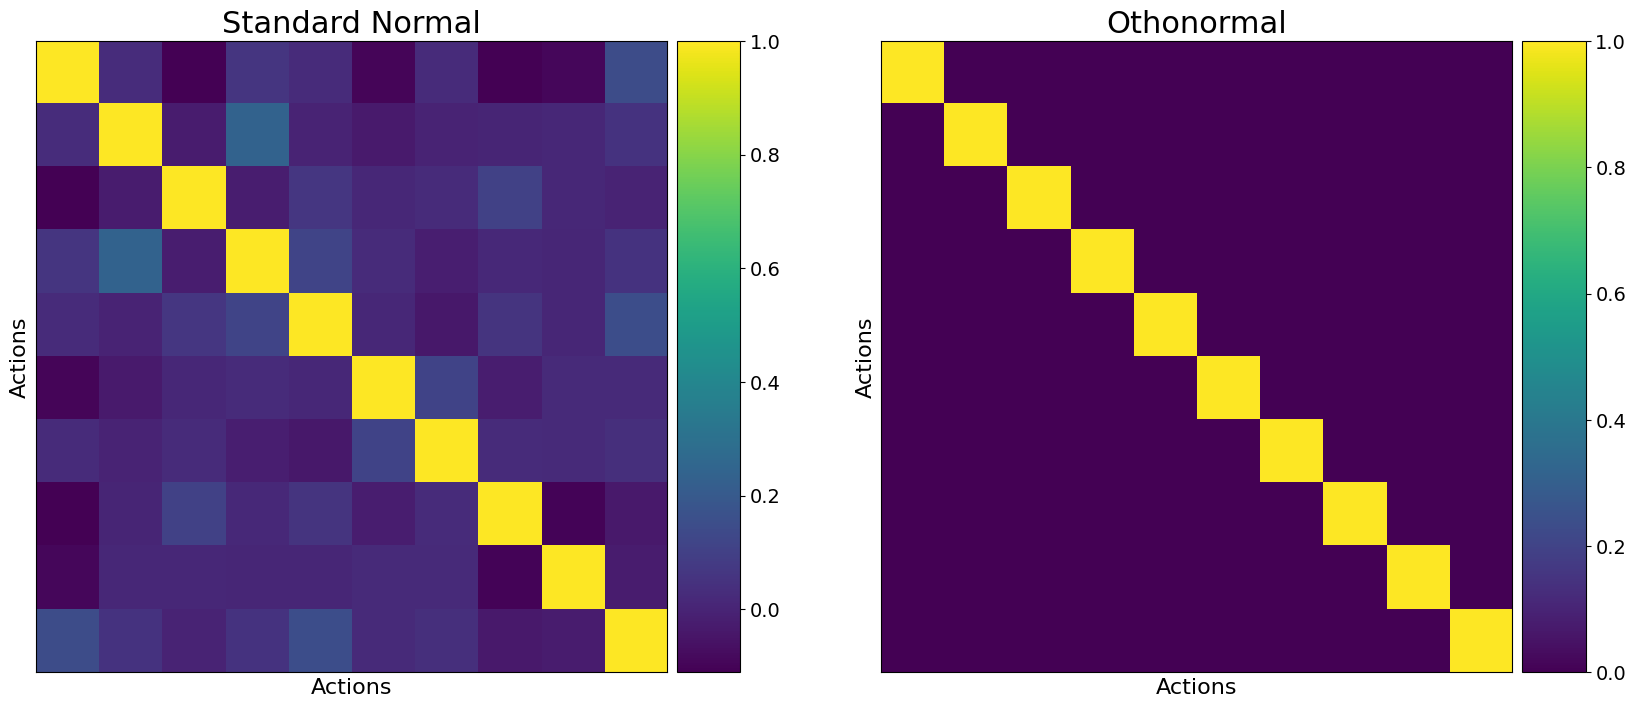
\includegraphics[width=\linewidth]{images/act_sims_128.png}
        \caption{}
        \label{fig:act_sims_128}
    \end{subfigure}
    \begin{subfigure}{0.58\textwidth}
        \centering
        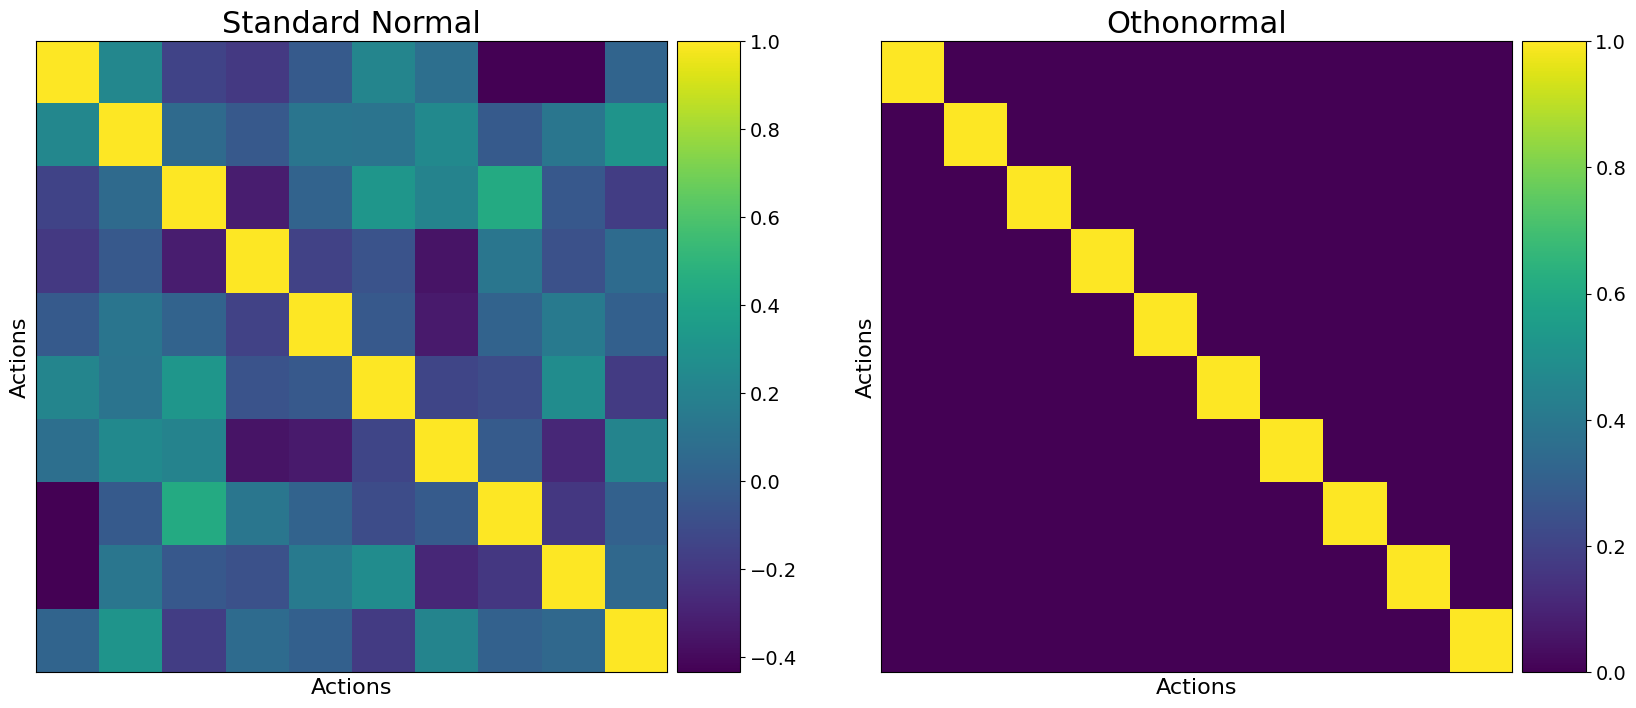
\includegraphics[width=\linewidth]{images/act_sims_16.png}
        \caption{}
        \label{fig:act_sims_16}
    \end{subfigure}
    \begin{subfigure}{0.58\textwidth}
        \centering
        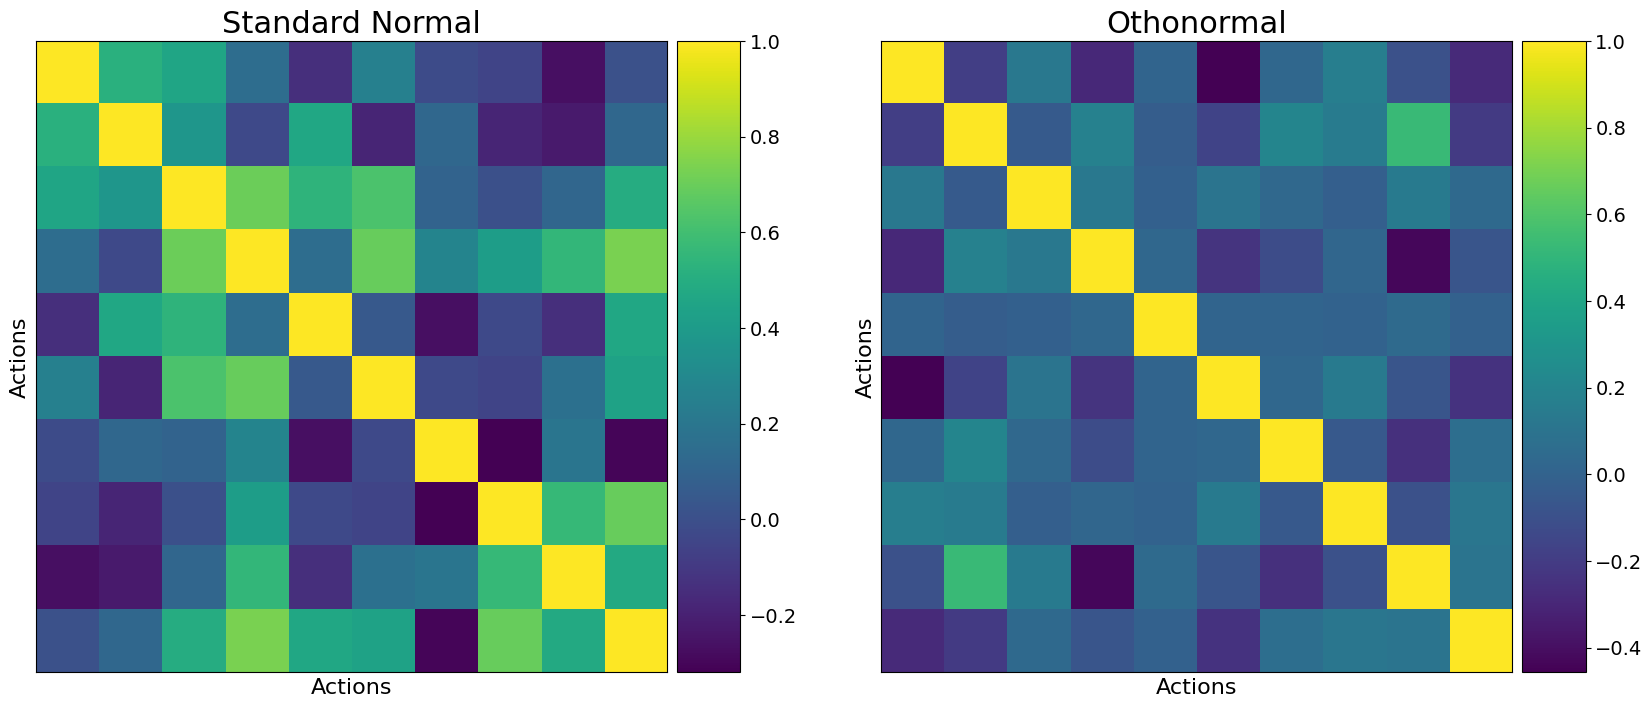
\includegraphics[width=\linewidth]{images/act_sims_more.png}
        \caption{}
        \label{fig:act_sims_more}
    \end{subfigure}
    \caption{These plots illustrate the pairwise cosine similarities between action embeddings for orthonormal versus standard normal distributions. (a) In a $128$-dimensional space with $10$ actions, orthonormal embeddings exhibit perfect decorrelation, whereas standard normal embeddings display non-zero similarities among them. (b) With $10$ actions in a $16$-dimensional space, the similarity between embeddings increases as the dimensionality of the space decreases, indicating denser correlations. (c) For $10$ actions in an $8$-dimensional space, despite the action count exceeding the space's dimensionality, orthonormal vectors (referenced in Appendix: Orthonormal Vectors) maintain lower similarities compared to those from a standard normal distribution, emphasizing the robustness of orthonormal embeddings in constrained dimensions.}
    \label{fig:act_sims_types}
    \vskip -0.2in
\end{figure*}
